\documentclass{article}

\title{Programmazione di Sistema: OS Internals}
\date{2022-09-28}
\author{Manuel Cadeddu}
\usepackage[italian]{babel}
\usepackage{amsmath}
\usepackage{graphicx}
\usepackage{subcaption}
\usepackage{setspace}
\usepackage{xcolor} 


\begin{document}
	\pagenumbering{arabic}
	\maketitle
	\newpage
	\doublespacing
	\tableofcontents
	\singlespacing
	\newpage
	
	\section{Main Memory}

		\subsection{Introduzione}

			\subsubsection{Hardware di Base}
				La Memoria consiste in un array di byte identificati da un indirizzo.
				\\La CPU può accedere solamente alla \textbf{Memoria Centrale} (RAM) e ai \textbf{Registri}, ma non al \textbf{Disco}. Quindi, tutte le istruzioni in esecuzione e i dati che utilizzano devono essere caricati in Memoria prima che la CPU possa operare su essi.
				\\I Registri hanno una memoria molto piccola e veloce ed è possibile accedervi con un solo colpo di clock. Invece, per accedere alla Memoria sono necessari più colpi di ck e questo può causare \textit{stalli}. Per migliorare la situazione sono state introdotte le \textbf{Cache}: buffer di memoria veloce che si trovano nel processore e permettono di non accedere in memoria (se possiedono i dati cercati).
				\\Un problema da gestire è quello di permettere ad un processo di accedere solo alla memoria per la quale è autorizzato. Per farlo si usano solitamente implementazioni hw, perché il SO non interviene negli accessi della CPU alla memoria per motivi di prestazioni.
				\\Una tecnica per implementare questa protezione è quella di avere due registri nella CPU: il \textbf{Base Register} e il \textbf{Limit Register}. Il Base Register contiene l'indirizzo minimo accedibile dal processo, il Limit Register la porzione di memoria assegnata al processo e, insieme, definiscono lo spazio degli \textit{Indirizzi Logici}. Quando la CPU deve accedere alla memoria verifica che l'indirizzo sia compreso tra il Base e Base + Limit. Se un processo cerca di accedere a un indirizzo non valido, viene generata una \textit{trap} che restituisce il controllo al SO per gestirla.
				\begin{figure}[ht!]
					\centering{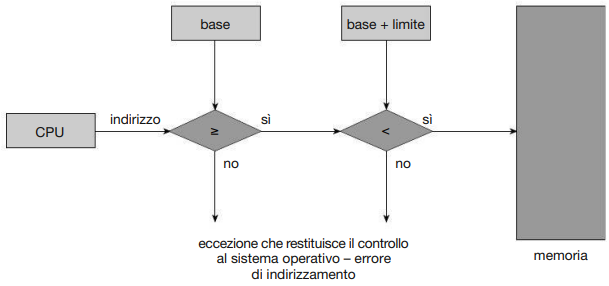
\includegraphics[width=12cm,height=5cm,keepaspectratio]{ch9_1.png}}
				\end{figure}
				\\I Base e Limit Register sono modificabili solo tramite \textit{istruzioni privilegiate} che possono essere eseguite solo in modalità kernel e, poiché solo il SO può essere eseguito in tale modalità, i processi utente non possono modificare il loro valore.

			\newpage
			\subsubsection{Fasi di Elaborazione di un Programma}
				Vediamo i vari componenti che permettono ad un file sorgente di diventare un eseguibile e di essere caricato in RAM per essere eseguito:
				\begin{itemize}
					\item \textbf{preprocessore}: spesso considerato parte del compilatore, permette l'inclusione di header files, di espandere macro, di eseguire compilazione condizionale\dots 
					\\In output si ha un altro file C;
					\item \textbf{compilatore}: traduce il C in linguaggio macchina e produce un \textit{file oggetto} per ogni file C;
					\item \textbf{linker}: unisce i file oggetto e le librerie statiche per creare un \textit{file eseguibile} (\textit{loadable image});
					\item \textbf{loader}: copia la \textit{loadable image} in Memoria, connettendola con librerie dinamiche.
				\end{itemize}
				\begin{figure}[ht!]
					\centering{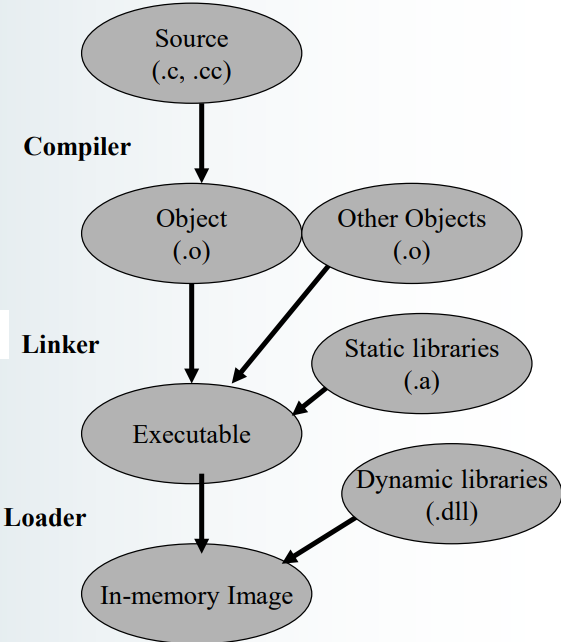
\includegraphics[width=12cm,height=5.5cm,keepaspectratio]{ch9_2.png}}
				\end{figure}
			
			\subsubsection{Address Binding}
				L'Address Binding si rifferisce alla mappatura delle istruzioni e dei dati in posizioni di memoria fisica.
				\\Generalmente, gli indirizzi nel file sorgente sono simbolici (es. nomi variabili), il compilatore associa questi indirizzi simbolici a indirizzi rilocabili (es. 14 byte dall'inizio di questo modulo) e, infine, il linker o il loader genera gli indirizzi assoluti (es. 7014 byte dall'inizio della memoria). Ogni associazione rappresenta una corrispondenza da uno spazio d'indirizzi a un'altro.
				\\Esistono tre tipi di address binding:
				\begin{itemize}
					\item \textbf{Compile Time Address Binding}: se il compilatore sa dove il processo risiederà in memoria, può generare \textbf{codice assoluto}. In questo caso, se dovesse cambiare la locazione iniziale, bisognerebbe ricompilare il codice;
					\item \textbf{Load Time Address Binding}: se in fase di compilazione non è possibile sapere in che punto della memoria risiederà il processo, il compilatore genera \textbf{codice rilocabile}. In questo caso il \textit{codice assoluto} viene generato in fase di caricamento e, se cambia l'indirizzo del processo, è sufficiente ricaricare il codice per ottenere il nuovo indirizzo "base";
					\item \textbf{Execution Time Address Binding}: se durante l'esecuzione il processo può essere spostato in memoria, si deve ritardare la generazione degli \textit{indirizzi assoluti} fino alla fase di esecuzione. La maggior parte dei SO usa questa soluzione.
				\end{itemize}
		
			\subsubsection{Spazi di Indirizzi Logici e Fisci}
				Un indirizzo generato dalla CPU è normalmente chiamato \textbf{indirizzo logico}, mentre quello caricato nel rigistro dell'indirizzo di memoria è chiamato \textbf{indirizzo fisico}.	
				\\I metodi di associazione degli indirizzi in fase di compilazione e di caricamento producono indirizzi logici e fisici identici. Con l'associazione in fase di esecuzione gli indirizzi logici non coincidono con quelli fisici. In questo caso ci si riferisce agli indirizzi logici col termine \textbf{indirizzi virtuali}.
				\\L'insieme degli indirizzi logici generati da un programma è lo \textbf{spazio degli indirizzi logici}; l'insieme degli indirizzi fisici corrispondenti a tali indirizzi logici è lo \textbf{spazio degli indirizzi fisci}.
				\\Per implementare l'Execution Time Address Binding,  l'associazione dagli indirizzi virtuali a quelli fisici è svolta da un dispositivo (interno alla CPU) detto \textbf{MMU} (\textbf{Memory Management Unit}). Come vedremo più avanti, questo binding può essere realizzato in diversi modi. Per esempio, sommando l'indirizzo logico al contenuto del registro base (ora chimato \textbf{relocation register}).
				\begin{figure}[ht!]
					\centering{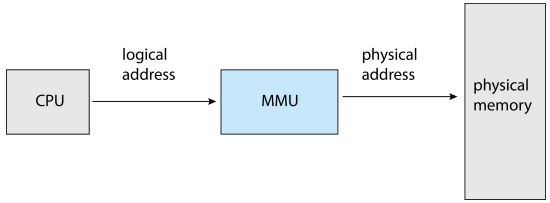
\includegraphics[width=12cm,height=3.5cm,keepaspectratio]{ch9_3.png}}
				\end{figure}

			\subsubsection{Dynamic Loading}
				Nella discussione svolta fin’ora, era necessario che l’intero programma e i dati di un processo fossero presenti nella memoria fisica perché il processo potesse essere eseguito. Per migliorare l’utilizzo della memoria si può ricorrere al \textbf{caricamento dinamico} (dynamic loading), mediante il quale si carica una procedura solo quando viene richiamata; tutte le procedure si tengono su disco in un formato di caricamento rilocabile. Si carica il programma principale in memoria e quando una procedura deve richiamarne un’altra, controlla innanzitutto che sia stata caricata. Se non è stata caricata, caricare in memoria la procedura richiesta e aggiornare le tabelle degli indirizzi del programma. A questo punto il controllo passa alla procedura appena caricata.
				\\Il caricamento dinamico non richiede un supporto particolare del SO. Spetta agli utenti progettare i programmi in modo da trarre vantaggio da un metodo di questo tipo. Il SO può tuttavia aiutare il programmatore fornendo librerie di procedure che realizzano il caricamento dinamico.
			

			\subsubsection{Dynamic Linking e Librerie Condivise}
				Le \textbf{Dynamically Linked Libraries} (\textbf{DLLs}, librerie caricate dinamicamente) sono librerie di sistema che vengono collegate ai programmi utente quando questi vengono eseguiti. Alcuni SO consentono solo il collegamento statico (static linking), in cui le librerie di sistema sono trattate come qualsiasi altro modulo oggetto e combinate dal caricatore nell’immagine binaria del programma. Il concetto di linking dinamico, invece, è analogo a quello di dynamic loading. Invece di differire il caricamento di una procedura fino al momento dell’esecuzione, si differisce il collegamento. Questa caratteristica si usa soprattutto con le librerie di sistema, per esempio le librerie di subroutine del linguaggio. Senza questo strumento tutti i programmi di un sistema dovrebbero disporre, all’interno dell’eseguibile, di una copia della libreria di linguaggio (o almeno delle procedure cui il programma fa riferimento). Tutto ciò spreca spazio nei dischi e in memoria centrale.
				\\Con il linking dinamico, invece, per ogni riferimento a una procedura di libreria s’inserisce all’interno dell’eseguibile una piccola porzione di codice di riferimento (\textbf{stub}), che indica come localizzare la giusta procedura di libreria residente in memoria o come caricare la libreria se la procedura non è già presente. Durante l’esecuzione, lo stub controlla se la procedura richiesta è già in memoria, altrimenti provvede a caricarla; in entrambi i casi lo stub sostituisce se stesso con l’indirizzo della procedura, che viene poi eseguita. In questo modo, quando si raggiunge nuovamente quel segmento del codice, si esegue direttamente la procedura di libreria, senza costi aggiuntivi per il linking dinamico. Con questo metodo tutti i processi che usano una libreria del linguaggio eseguono la stessa copia del codice della libreria. Questo sistema è noto anche con il nome di \textbf{librerie condivise}.
				\\A differenza del caricamento dinamico, il linking dinamico e le librerie condivise richiedono generalmente l’assistenza del sistema operativo. Se i processi presenti in memoria sono protetti l’uno dall’altro, il sistema operativo è l’unica entità che può controllare se la procedura richiesta da un processo è nello spazio di memoria di un altro processo, o che può consentire l’accesso di più processi agli stessi indirizzi di memoria.

		\subsection{Allocazione Contigua della Memoria}
			La memoria centrale deve contenere sia il SO che i vari processi, quindi bisogna gestirla in modo efficiente. Vediamo ora la prima tecnica per l'allocazione della memoria: l'\textbf{allocazione contigua della memoria}.
			\\La RAM viene di solito divisa in due partizioni, una per il SO e una per i processi. Poiché l'IVT si trova solitamente agli indirizzi inferiori, anche il SO viene allocato agli indirizzi più bassi.
			\\Con l’allocazione contigua della memoria, ciascun processo è contenuto in una singola sezione di memoria contigua a quella che contiene il processo successivo. Per assicurarsi che si acceda alla memoria corretta è possibile utilizzare i registri Base e Limit:
			\begin{figure}[ht!]
				\centering{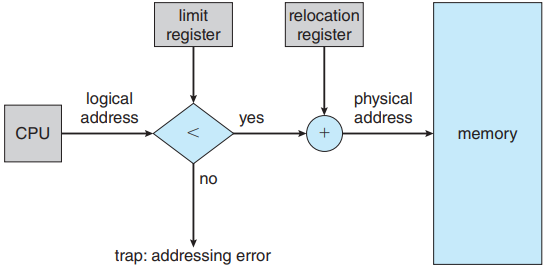
\includegraphics[width=12cm,height=4cm,keepaspectratio]{ch9_4.png}}
			\end{figure}
			\\L'utilizzo di questi registri può risultare util anche per cambiare dinamicamente la dimensione della memoria dedicata al processo (non sempre possibile).

			\subsubsection{Allocazione della Memoria}
				Uno dei metodi più semplici per l’allocazione della memoria consiste nel suddividere la stessa in partizioni di dimensione fissa.
				\\Nello schema a partizione variabile il SO conserva una tabella in cui sono indicate le partizioni di memoria disponibili e quelle occupate. Inizialmente
				tutta la memoria è a disposizione dei processi utenti; si tratta di un grande blocco di memoria disponibile, un buco (\textbf{hole}). Nel lungo periodo la memoria contiene una serie di buchi di diverse dimensioni.
				\begin{figure}[ht!]
					\centering{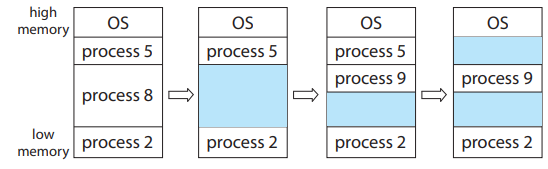
\includegraphics[width=12cm,height=3cm,keepaspectratio]{ch9_5.png}}
				\end{figure}
				\\Quando entrano nel sistema, i processi vengono inseriti in una coda d’ingresso. Per determinare a quali processi si debba assegnare la memoria, il SO tiene conto dei requisiti di memoria di ciascun processo e della quantità di spazio di
				memoria disponibile. Quando a un processo si assegna dello spazio, il processo stesso viene caricato in memoria e può quindi competere per il controllo della CPU. Al termine, rilascia la memoria che gli era stata assegnata, e il SO può impiegarla per un altro processo presente nella coda d’ingresso.
				\\I criteri più usati per scegliere un buco libero tra quelli disponibili nell’insieme sono i seguenti:
				\begin{itemize}
					\item \textbf{Firstfit}: si assegna il primo buco abbastanza grande. La ricerca può cominciare sia dall’inizio dell’insieme di buchi sia dal punto in cui era terminata la ricerca precedente. Si può fermare la ricerca non appena s’individua un buco libero di dimensioni sufficientemente grandi;
					\item \textbf{Bestfit}: si assegna il più piccolo buco in grado di contenere il processo. Si deve
					compiere la ricerca in tutta la lista, a meno che questa non sia ordinata per dimensione. Tale criterio produce le parti di buco inutilizzate più piccole;
					\item \textbf{Worstfit}: si assegna il buco più grande. Anche in questo caso si deve esaminare tutta la lista, a meno che non sia ordinata per dimensione. Tale criterio produce le	parti di buco inutilizzate più grandi, che possono essere più utili delle parti più
					piccole ottenute col criterio best-fit.
				\end{itemize}
				Con l’uso di simulazioni si è dimostrato che sia first-fit sia best-fit sono migliori rispetto a worst-fit in termini di risparmio di tempo e di utilizzo di memoria. D’altra parte nessuno dei due è chiaramente migliore dell’altro per quel che riguarda l’utilizzo della memoria ma, in genere, first-fit è più veloce.

			\subsubsection{Frammentazione}
				Si distinguono:
				\begin{itemize}
					\item \textbf{frammentazione esterna}: spazio libero in RAM tra i diversi processi;
					\item \textbf{frammentazione interna}: memoria non occupata dal processo che però è stata allocata per esso.
				\end{itemize}
				La frammentazione esterna dipende dalla dimensione della memoria e da quella dei processi ma è generalmente abbastanza grave. Con l'algoritmo first-fit, per esempio, l'analisi statistica rivela che per \textit{n} blocchi, si perdono circa 0.5*\textit{n} blocchi (\textbf{regola del 50 per cento}), ovvero 1/3 della memoria non viene usato.
				\\Un metodo per migliorare il problema della frammentazione esterna è quello della \textbf{compattazione}: si spostano i blocchi di memoria dedicati ai processi creando un unico grande blocco. Questo però non deve essere possibile solo in fase di assemblaggio o loading, ma anche mentre i processi sono in esecuzione (in READY). Quindi gli indirizzi devono essere rilocabili dinamicamente. Se lo sono, la rilocazione richiede solo lo spostamento del programma e dei dati, e quindi la modifica del registro di rilocazione in modo che possieda il nuovo Base Register. La compattazione può però generare il \textit{problema I/O}, ovvero se un processo viene spostato mentre è in WAIT, in attesa di un operazione di I/O, la scrittura/lettura può essere fatta nella porzione di memoria sbagliata. Per risolvere questo problema sono possibili due soluzioni: impedire lo spostamento di processi che stanno eseguendo operazioni I/O o utilizzare dei buffer del SO, non soggetti a reallocazione, come intermediari tra la memoria e i dispositivi I/O.
				\\L'algoritmo di compattazione più semplice consiste nello spostare tutti i processi verso un'estremità della memoria e può essere assai oneroso. 
				\\Altre due tecniche usate per evitare la frammentazione esterna sono la \textbf{segmentazione} e la \textbf{paginazione} (queste tecniche si possono combinare).

		\subsection{Paginazione}
			La paginazione è una tecnica che permette l'assegnazione di blocchi di memomoria non contigui ad un processo. La paginazione evita la frammentazione esterna e la necessità di compattare perché non c'è più il problema di avere blocchi di memoria di dimensioni variabili. 
			\\Il metodo di base consiste nello suddividere la \underline{memoria fisica} in blocchi di dimensione fissa, chiamati \textbf{frame}, e la \underline{memoria logica} in blocchi della stessa dimensione (dei frame), detti \textbf{pagine}. Quando si deve eseguire un processo, si caricano le sue pagine nei frame disponibili, prendendole dalla memoria ausiliaria o dal file system. Questa tecnica fornisce grandi funzionalità. Per esempio, ora lo spazio degli indirizzi logici è totalmente separato dallo spazio degli indirizzi fisici e dunque un processo può avere uno spazio degli indirizzi logici a 64 bit anche se il sistema ha meno di $2^{64}$ byte di memoria fisica.
			\\Gli indirizzi logici vengono divisi in \textbf{page number} (\textbf{p}) e \textbf{page offset} (\textbf{d} = displacement). Il \textit{page number} serve come indice per la \textbf{paging table}, contenente l'indice del frame, che viene usato per calcolare l'indirizzo fisico.
			\\L'hardware di supporto è il seguente:
			\begin{figure}[ht!]
				\centering{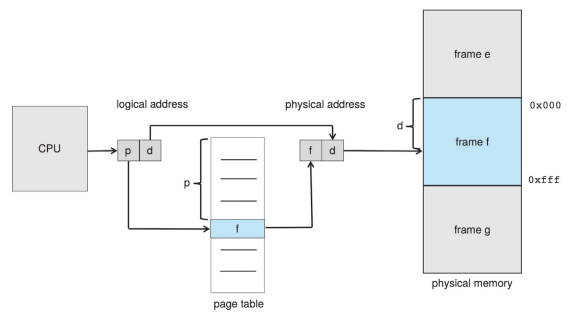
\includegraphics[width=12cm,height=6.5cm,keepaspectratio]{ch9_6.png}}
			\end{figure}
			\\La dimensione di una pagina, così come quella di un frame, è definita dall’hardware ed è, in genere, una potenza di 2 compresa tra 512 byte e 1 Gb. La scelta di una potenza di 2 facilita la traduzione di un indirizzo logico nei corrispondenti numero e offset di pagina. Se la dimensione dello spazio degli indirizzi logici (dimensione memoria logica) è \textit{$2^{m}$} byte (servono indirizzi di \textit{m} bit per identificare un determinato byte) e la dimensione di una pagina è di \textit{$2^{n}$} byte (servono indirizzi di n bit per identificare un determinato byte), per identificare una pagina servono indirizzi di \textit{m} - \textit{n} bit ($2^{m}$/$2^{n}$ pagine).
			\\L’indirizzo logico ha quindi la seguente forma:
			\begin{figure}[ht!]
				\centering{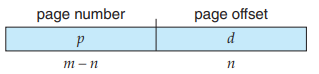
\includegraphics[width=12cm,height=1.3cm,keepaspectratio]{ch9_8.png}}
			\end{figure}
			\\dove \textit{p} è un indice della tabella delle pagine e
			\textit{d} è l’offset all’interno della pagina.
			\\Vediamo un esempio. Consideriamo la seguente memoria:
			\begin{figure}[ht!]
				\centering{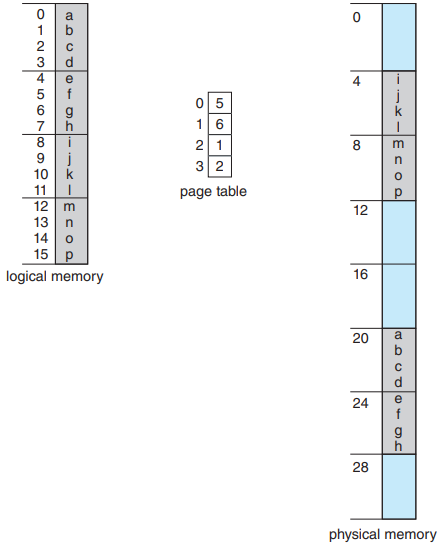
\includegraphics[width=12cm,height=6cm,keepaspectratio]{ch9_9.png}}
			\end{figure}
			\\Possiamo osservare che: \textit{m} = 4, \textit{n} = 2 e che la memoria fisica può contenere 8 frame. Per ottenere l'indirizzo fisico si calcola \textit{f} moltiplicando il numero di pagina indicato nella tabella delle pagine per la dimensione della pagina e si somma \textit{d} al risutato.

			\subsubsection{Frammentazione Interna}
				Con la paginazione si evita la frammentazione esterna ma non quella interna. Infatti, poiché la dimensione dei processi solitamente non è un multiplo di quella dei frame, l'ultimo frame può essere riempito solo parzialmente:
				\begin{itemize}
					\item caso migliore: 0 byte;
					\item caso peggiore: dim\_frame - 1 byte;
					\item caso medio: dim\_frame/2;
				\end{itemize}
				Da queste considerazioni possiamo osservare che più le pagine sono piccole, minore è la frammentazione interna ma maggiore è la dimensione della page table. Attualmente la dimensione tipica delle pagine è compresa tra 4 e 8 KB.

			\subsubsection{Struttura Entry della Page Table}
				La entry di una Page Table mantiene le seguenti informazioni:
				\begin{figure}[ht!]
					\centering{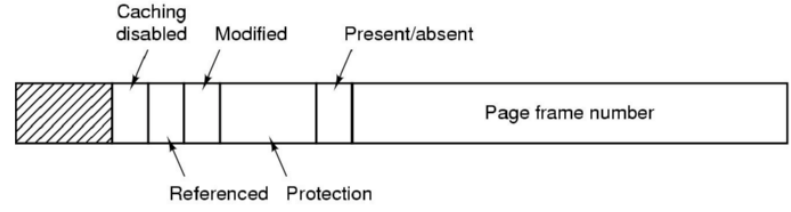
\includegraphics[width=12cm,height=2.7cm,keepaspectratio]{ch9_10.png}}
				\end{figure}
				\\Poiché la Page Table è troppo grande per essere nella CPU, viene memorizzata in RAM. Nella CPU sono invece presenti due registri:
				\begin{itemize}
					\item \textbf{Page-Table Base Register} (\textbf{PTBR}): indirizzo base della Page Table in RAM;
					\item \textbf{Page-Table Length Register} (\textbf{PTLR}): dimensione della Page Table;
				\end{itemize}
				Notare che l'utilizzo di questa tecnica richiede due accessi a memoria per accedere all'istruzione/dato (uno per tradurre indirizzo logico in fisico e uno per eseguire l'operazione). Questo dimezza la velocità della memoria. Per risolvere questo problema può essere usata una cache ad accesso diretto (CAM o Memoria Associativa) detta \textbf{Translaction Lookaside Buffers} (\textbf{TLB}). La memoria associativa è progettata in modo che si possa effettuare ricerca in parallelo su tutte le entry e solo la entry che matcha (se presente e massimo una) produce l'output desiderato. Essendo una cache può esserci \textit{TLB miss} ma comunque migliora le prestazioni. 
				\begin{figure}[ht!]
					\centering{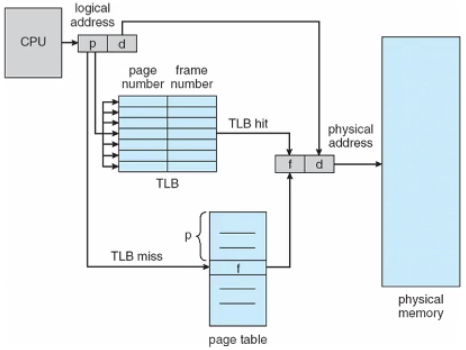
\includegraphics[width=12cm,height=5cm,keepaspectratio]{ch9_12.png}}
				\end{figure}
				\newpage
				\noindent La TLB è solitamente piccola, da 64 a 1024 entry.
				\begin{figure}[ht!]
					\centering{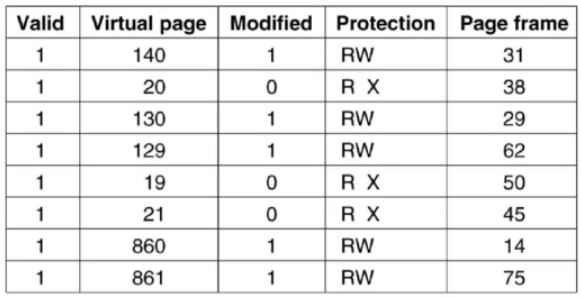
\includegraphics[width=12cm,height=4cm,keepaspectratio]{ch9_11.png}}
				\end{figure}
				\\Vediamo come può essere calcolato l'\textbf{Effective Access Time} (\textbf{EAT}): ipotizziamo di avere un \textit{hit ratio} dell'80\% e che il tempo di accesso alla memoria in caso di \textit{TLB hit} sia di 10 ns (quindi di 20 ns in caso di miss):
				\begin{itemize}
					\item EAT = 0.8 * 10 + 0.2 * 20 = 12 ns
				\end{itemize}

			\subsubsection{Protezione}
				In un ambiente paginato, la protezione della memoria è assicurata dai \textbf{bit di protezione} associati a ogni frame; normalmente tali bit si trovano nella tabella delle pagine (e nella TLB) e sono usati, ad esempio, per determinare se una pagina si può leggere e scrivere oppure soltanto leggere. 
				\\Quando si interroga la page table per calcolare l’indirizzo fisico, vengono controllati i bit di protezione per verificare che non si scriva in una pagina di sola lettura. Un tale tentativo causerebbe la generazione di un’eccezione hardware per il SO. Questo metodo si può facilmente estendere per fornire un livello di protezione più perfezionato aggiungendo bit.
				\\Di solito si associa a ciascun elemento della tabella delle pagine un ulteriore bit, detto \textbf{bit di validità}. Tale bit, impostato a valido, indica che la pagina corrispondente è nello spazio d’indirizzi logici del processo, quindi è una pagina valida. Il bit di validità consente quindi di riconoscere gli indirizzi illegali e di notificarne la presenza attraverso un’eccezione.
				\newpage
				\noindent Per esempio, supponiamo che in un sistema con uno spazio di indirizzi di 14 bit (da 0 a 16.383) si abbia un programma che deve usare soltanto gli indirizzi da 0 a 10.468 e che le pagine sono di 2 kB.
				\begin{figure}[ht!]
					\centering{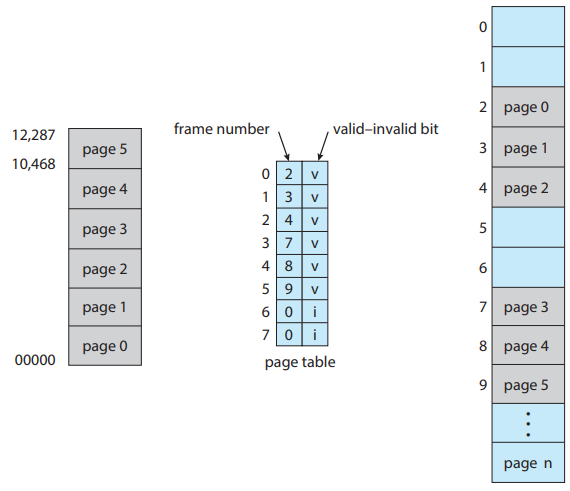
\includegraphics[width=12cm,height=6.5cm,keepaspectratio]{ch9_13.png}}
				\end{figure}
				\\Gli indirizzi nelle pagine 0, 1, 2, 3, 4 e 5 sono tradotti normalmente tramite la tabella delle pagine. D’altra parte, ogni tentativo di generare un indirizzo nelle pagine 6 o 7 trova il bit di validità non valido; in questo caso il calcolatore invia un’eccezione al sistema operativo (riferimento di pagina non valido).
				\\Questo schema ha creato un problema: poiché il programma si estende solo fino all’indirizzo 10.468, ogni riferimento oltre tale indirizzo è illegale; i riferimenti alla pagina 5 sono tuttavia classificati come validi, e ciò rende validi gli accessi sino all’indirizzo 12.287; solo gli indirizzi da 12.288 a 16.383 sono non validi. Tale problema è dovuto alla dimensione delle pagine di 2 kb e corrisponde alla frammentazione interna della paginazione.
			
			\subsubsection{Pagine Condivise}
				Un altro vantaggio della paginazione consiste nella possibilità di condividere pagine  tra processi, con conseguente risparmio di RAM.
				\\Se una pagina di codice (es. funzione di libreria) deve essere condivisa, deve contenere \textbf{codice rientrante}. Il codice rientrante non cambia durante l’esecuzione. Quindi, due o più processi possono eseguirlo nello stesso momento. I dati usati da queste funzioni sono invece tipicamente privati.
				\\Si consideri un sistema con 40 utenti, ciascuno dei quali usa un text editor. Se tale programma è formato da 150 kb di codice e 50 kB di spazio di dati, per gestire i 40 utenti sono necessari 8000 kB. Se invece il codice viene condiviso sono necessari solo 2150 kB.
				\newpage
				\begin{figure}[ht!]
					\centering{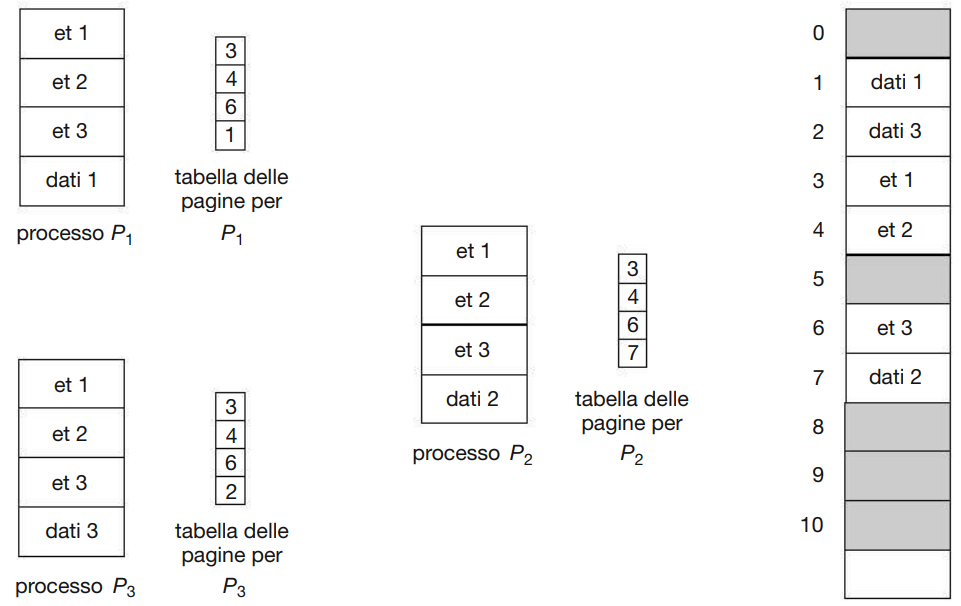
\includegraphics[width=12cm,height=6.5cm,keepaspectratio]{ch9_14.png}}
				\end{figure}
				\noindent Il codice condiviso è read-only ma possono essere condivise anche pagine di dati read/write per permettere la comunicazione tra processi.

		\subsection{Struttura della Page Table}
			La tabella delle pagine potrebbe diventare enorme. Considerariamo ad esempio uno spazio di indirizzamento logico a 32 bit e pagine di 4kB. La tabella delle pagine dovrebbe avere circa 1 milione di entry ($2^{32}/2^{12}$) e, se ogni entry è di 4 B, ogni processo occuperebbe 4 MB di memoria fisica solo per essa. Inoltre, bisogna notare che la memoria occupata dovrebbe essere contigua perché la tabella viene usata come un array ad accesso diretto.
			\\Quello che vogliamo fare è  eliminare il problema della contiguità della memoria. Vediamo alcune delle tecniche più comuni usate per strutturare la tabella delle pagine:
			\begin{itemize}
				\item \textbf{paginazione gerarchica};
				\item \textbf{hashed page table};
				\item \textbf{inverted page table}.
			\end{itemize}

			\newpage
			\subsubsection{Paginazione Gerarchica}
				La paginazione gerarchica è una soluzione semplice per evitare di collocare la page table in modo contiguo in RAM. Questo metodo consiste nell’adottare un algoritmo di paginazione a più livelli, in cui la tabella stessa è paginata. 
				\begin{figure}[ht!]
					\centering{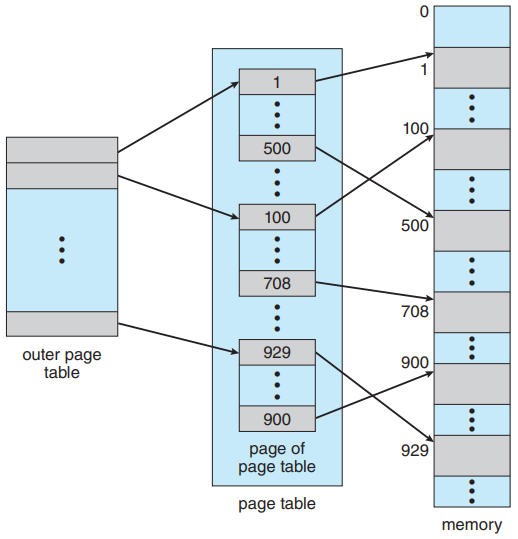
\includegraphics[width=12cm,height=6cm,keepaspectratio]{ch9_15.png}}
				\end{figure}
				\\Si consideri l'esempio di macchina a 32 bit con dimensione delle pagine di 4 kB ed entry nella page table di 4 byte. Ciascun indirizzo logico è suddiviso in un numero di pagina di 20 bit e in un offset di pagina di 12. Paginando la tabella delle pagine (4 MB in pagine da 4 kB), anche il numero di pagina è suddiviso in un numero di pagina di 10 bit e un offset di 10 (una entry occupa 4 byte, quindi non c'è bisogno di accedere a ogni byte ma ad uno ogni 4).
				\begin{figure}[ht!]
					\centering{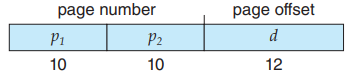
\includegraphics[width=12cm,height=1.2 cm,keepaspectratio]{ch9_16.png}}
				\end{figure}
				\\Poiché la traduzione degli indirizzi si svolge dalla tabella esterna delle pagine verso l’interno, questo metodo è anche noto come \textbf{tabella delle pagine ad associazione diretta} (\textbf{forward-mapped page table}).
				\\Tra gli svantaggi che possiamo notare c'è la maggiore occupazione di memoria (overhead) e il dover effettuare un ulteriori accessi all a RAM.
				\\La paginazione a due livelli non è adatta per sistemi con uno spazio di indirizzi logici a 64 bit. Si supponga che la dimensione delle pagine di questo sistema sia di 4 kB. In questo caso, la tabella delle pagine conterrà fino a $2^{52}$ elementi. Adottando uno schema di paginazione a due livelli, le page table interne possono occupare una pagina, o contenere $2^{10}$ elementi di 4 byte. 
				\begin{figure}[ht!]
					\centering{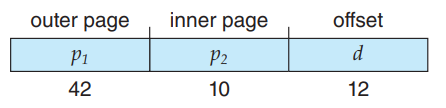
\includegraphics[width=12cm,height=1.3cm,keepaspectratio]{ch9_17.png}}
				\end{figure}
				\\La page table esterna è di $2^{42}$ elementi. La soluzione per evitare una tabella tanto grande consiste nel suddividerla in parti più piccole. Per esempio, si può paginare ottenendo uno schema di paginazione a tre livelli. Si supponga che la tabella esterna delle pagine sia costituita di pagine di dimensione ordinaria ($2^{10}$ elementi, o $2^{12}$ byte); uno spazio d’indirizzi a 64 bit è ancora enorme:
				\begin{figure}[ht!]
					\centering{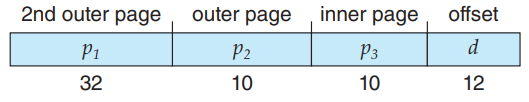
\includegraphics[width=12cm,height=1.3cm,keepaspectratio]{ch9_18.png}}
				\end{figure}
				\\Il passo successivo sarebbe uno schema di paginazione a quattro livelli, in cui si pagina anche la tabella esterna di secondo livello delle pagine, e così via.

			\subsubsection{Hashed Page Table}
				Un metodo per gestire spazi d’indirizzi oltre i 32 bit consiste nell’impiego di una hash table, in cui l’argomento della funzione hash è il numero della pagina virtuale. Ogni elemento della tabella contiene una lista concatenata di elementi che la funzione di hash fa corrispondere alla stessa locazione ed è composto da tre campi: (1) numero della pagina virtuale, (2) indirizzo del frame corrispondente alla pagina virtuale e (3) puntatore al successivo elemento della lista.
				\\Algoritmo: si applica la funzione hash al numero della pagina virtuale contenuto nell’indirizzo virtuale, identificando un elemento della tabella. Si confronta il numero di pagina virtuale con il campo (1) del primo elemento della lista concatenata: se i valori coincidono, si usa il campo 2 per generare l’indirizzo fisico altrimenti, vengono esaminati gli elementi successivi.
				\begin{figure}[ht!]
					\centering{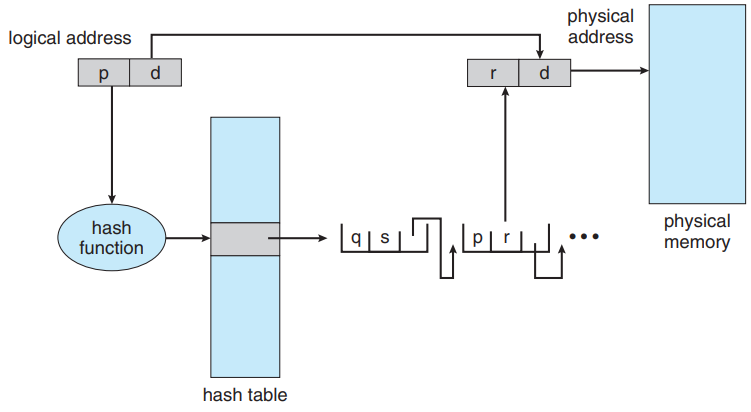
\includegraphics[width=12cm,height=5cm,keepaspectratio]{ch9_19.png}}
				\end{figure}
				\\Per questo schema è stata proposta una variante: la \textbf{page table a gruppi} (\textbf{clustered page table}), simile alla hash page table ma ciascun elemento della hash table contiene i riferimenti alle pagine fisiche corrispondenti a un gruppo di pagine virtuali contigue (per esempio 16). Queste tabelle sono particolarmente utili per gli spazi d’indirizzi sparsi, in cui i riferimenti alla memoria non sono contigui.

			\subsubsection{Inverted Page Table}
				Generalmente, si associa una tabella delle pagine a ogni processo e tale tabella contiene un elemento per ogni pagina virtuale che il processo sta usando. Uno degli inconvenienti di questo metodo è che ciascuna page table può occupare grandi quantità di memoria fisica.
				\\Per risolvere questo problema si può fare uso della tabella delle pagine invertita. Una inverted page table ha un elemento per ogni frame. Ciascun elemento è costituito dell’indirizzo virtuale della pagina memorizzata in quella reale locazione di memoria (\textit{p}) e dal \textit{pid} del processo che possiede tale pagina (perché processi diversi possono usare lo stesso \textit{p}). Quindi, nel sistema esiste una sola tabella delle pagine che ha un solo elemento per ciascuna pagina di memoria fisica. Se avviene il match con l'\textit{i-esima} entri, \textit{i} corrisponde all'indirizzo fisico.
				\begin{figure}[ht!]
					\centering{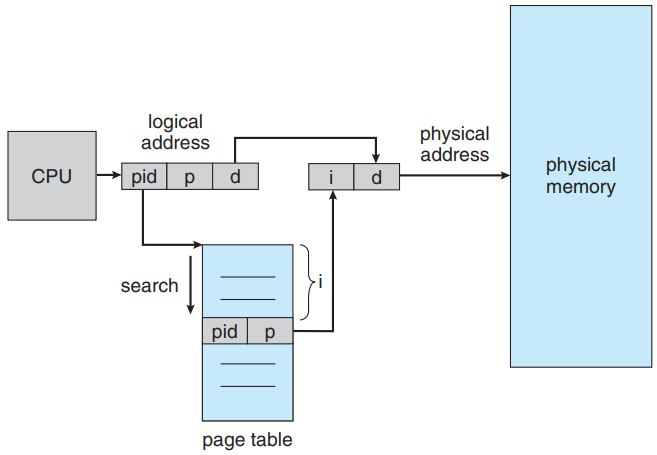
\includegraphics[width=12cm,height=5cm,keepaspectratio]{ch9_20.png}}
				\end{figure}
				\\I vantaggi di questa tecnica sono che la page table ha dimensione minori (dipenda dal numero di frame, non dalla dimensione dello spazio di indirizzamenti virtuale) e che c'è una unica tabella per tutti i processi (ogni frame è associato a un solo processo). Lo svantaggio è che non si ha accesso diretto (serve ricerca) e questo causa rallentamenti. Per eliminare questo problema le IPT sono associate a tabelle di hash.
				\begin{figure}[ht!]
					\centering{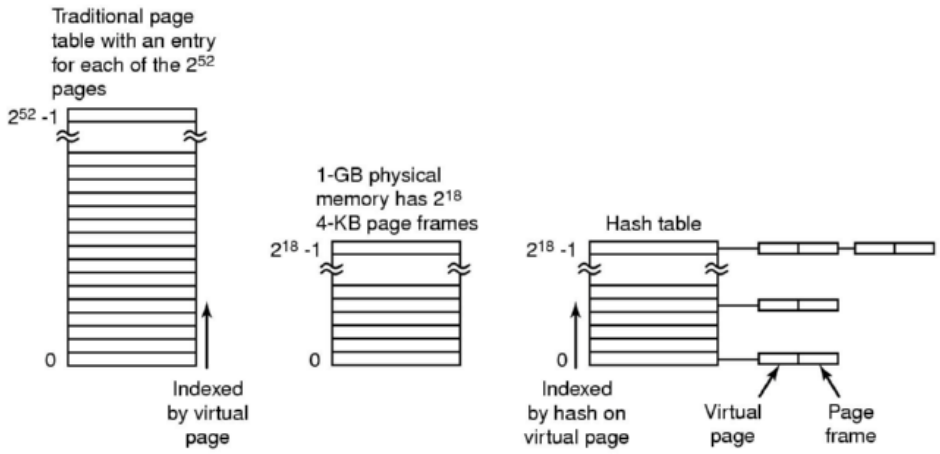
\includegraphics[width=12cm,height=5cm,keepaspectratio]{ch9_21.png}}
				\end{figure}
				
		\subsection{Swapping}
			Per essere eseguito, un processo deve trovarsi in RAM. Tuttavia, può essere temporaneamente tolto da essa (\textbf{swap/roll out}), essere spostato in una memoria ausiliaria (\textbf{backing store}) e in seguito riportato in memoria per continuare (\textbf{swap/roll in}) l’esecuzione. Questo procedimento si chiama avvicendamento dei processi in memoria (swapping). Grazie allo swapping lo spazio degli indirizzi fisici di tutti i processi può eccedere la reale dimensione della memoria fisica del sistema, aumentando il grado di multiprogrammazione possibile.
			\begin{figure}[ht!]
				\centering{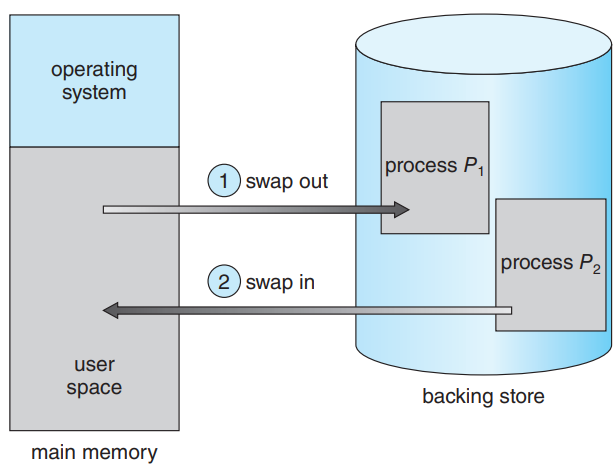
\includegraphics[width=12cm,height=5cm,keepaspectratio]{ch9_22.png}}
			\end{figure}

			\subsubsection{Standard Swapping}
				L’avvicendamento standard riguarda lo spostamento dei processi tra la RAM e backing store, di solito costituita da un disco veloce. Tale memoria deve essere abbastanza ampia da contenere le copie di tutte le immagini di memoria di tutti i processi utenti, e deve permettere un accesso diretto ad esse. Il sistema mantiene una coda dei processi pronti (\textit{ready queue}) formata dai processi pronti per l’esecuzione. Quando lo scheduler decide di eseguire un processo, richiama il dispatcher, che controlla se il primo processo della coda si trova in memoria centrale. Se non c'è, e in questa non c’è spazio libero, il dispatcher scarica un processo dalla memoria e vi carica il processo richiesto dallo scheduler, quindi ricarica i registri e trasferisce il controllo al processo selezionato.
				\\In un tale sistema d’avvicendamento, il tempo di context-switching è piuttosto elevato. Si pensi a un processo di 100 MB e a una memoria ausiliaria costituita da un normale hard disk con velocità di trasferimento di 50 MB al secondo. Il trasferimento del processo richiede: 100 MB / 50 MB al secondo = 2 secondi. Dal momento che dobbiamo scaricare e poi ricaricare il processo, il tempo totale è di circa 4 s.
				\\Occorre notare che la maggior parte del tempo d’avvicendamento è data dal tempo di trasferimento e che questo è direttamente proporzionale alla quantità di memoria trasferita. Perciò sarebbe utile sapere quanta memoria sia effettivamente usata da un processo e non solo quanta questo potrebbe usarne, poiché in questo caso è necessario trasferire solo quanto è effettivamente utilizzato, riducendo il tempo d’avvicendamento (\textbf{swapping con paging}). 
				\\Per scaricare un processo dalla memoria è necessario essere certi che sia completamente inattivo. Particolare importanza ha l’attesa di I/O: quando decidiamo di scaricare un processo per liberare la memoria, tale processo può essere nell’attesa del completamento di un’operazione di I/O. Tuttavia, se un dispositivo di I/O accede in modo asincrono alle aree di I/O della memoria (buffer) utente, il processo non può essere scaricato. Si supponga che l’operazione di I/O sia stata accodata, perché il dispositivo era occupato. Se il processo P2 s’avvicendasse al processo P1, l’operazione di I/O potrebbe tentare di usare la memoria che attualmente appartiene al processo P2. Questo problema si può risolvere in due modi: non scaricando dalla memoria un processo con operazioni di I/O pendenti, oppure eseguendo operazioni di I/O solo in buffer del SO. Trasferimenti fra tali aree del sistema operativo e la memoria assegnata al processo possono poi avvenire solo quando il processo è presente in RAM. Si noti che questo meccanismo di memorizzazione (\textbf{double buffering}) aggiunge overhead. Abbiamo infatti bisogno di copiare nuovamente i dati, dalla memoria del kernel alla memoria utente, prima che il processo utente possa accedervi.
				\\Attualmente l’avvicendamento nella sua forma standard si usa in pochi sistemi; richiede infatti un elevato tempo di trasferimento, e consente un tempo di esecuzione troppo breve per essere considerato una soluzione ragionevole al problema di gestione della memoria.

			\subsubsection{Swapping in Sistemi Mobili}
				Mentre la maggior parte dei SO per PC e server supporta qualche versione di swapping, i sistemi mobili in genere non ne supportano. Questi utilizzano solitamente, come memoria di massa, la memoria flash al posto dei dischi rigidi, più voluminosi. Il vincolo che ne deriva in termini di spazio è una delle ragioni per cui si evitalo swapping dei processi. Inoltre, vi sono il numero limitato di scritture che una memoria flash può sopportare prima di diventare inaffidabile e il trasferimento tra memoria centrale e memoria flash è lento.
				\\Invece di usare lo swapping, se la memoria disponibile scende al di sotto di una certa soglia, iOS di Apple chiede alle applicazioni di rinunciare volontariamente alla memoria allocata. I dati di sola lettura vengono rimossi dal sistema e successivamente ricaricati dalla memoria flash, se necessario. I dati che sono stati modificati (per esempio lo stack) non vengono rimossi. Tuttavia, tutte le applicazioni che non riescono a liberare memoria a sufficienza possono essere terminate dal SO.
				\\Android non supporta l’avvicendamento e adotta una strategia simile a quella di iOS. Anche Android può terminare un processo qualora la memoria libera disponibile non sia sufficiente. Tuttavia, prima di terminarlo, scrive lo stato dell’applicazione nella memoria flash, in modo che il processo possa essere rapidamente riavviato.
		

\end{document}